\chapter{Implementación}

Aunque en un primer momento me plantee implementar el algoritmo en Python encontré un  artículo\footnote{Juan-Julian Merelo-Guervós et al., Ranking the Performance of Compiled and Interpreted Languages in Genetic Algorithms, 2016} en el que nos indicaba que en base a su rendimiento dicho lenguaje no está aconsejado para implementar algoritmos genéticos recomendando entre otros el lenguaje Java que es el que finalmente utilicé por ser el que iba a darme mejores resultados y por la sencillez de uso de su biblioteca de clases.

\subsection{Representación de la solución}

La \textbf{representación} elegida ha sido una permutación de \texttt{n} elementos siendo \texttt{n} el número de localizaciones posibles. Dicha permutación está almacenada en un vector de enteros en el que el índice del vector indica la localización del elemento y el valor de dicha posición representa donde estará ubicada la instalación.

\subsection{Operadores}

\subsubsection{Operador de Selección}

Como \textbf{operador de selección} hemos realizado una selección por torneo. Se obtienen n individuos de forma aleatoria y se elige el mejor de ellos\footnote{\url{https://en.wikipedia.org/wiki/Tournament_selection}}.

\subsubsection{Operador de Cruce (OX2)}
El \textbf{operador de cruce} elegido para nuestro algoritmo ha sido el \texttt{OX2}\footnote{\url{https://en.wikipedia.org/wiki/Crossover_(genetic_algorithm)}}. Este operador permite que los hijos reciban la parte intermedia del cromosoma de uno de los padres, y el orden de los elementos de los extremos del otro padre. En la figura \ref{cruce_ox} podemos ver una representación gráfica de como se generan los genes de un hijo a partir de los de los padres.

\begin{figure}[ht!]
\centering
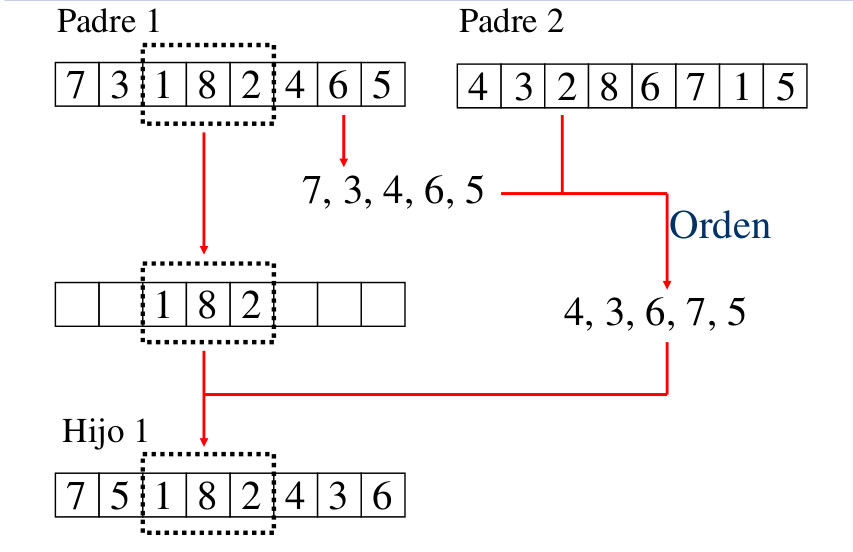
\includegraphics[width=220px]{../images/crossover_ox.jpg}
\caption{Operador de Cruce OX2 \label{cruce_ox}}
\end{figure}


En primer lugar se elige un rango central de elementos del cromosoma que se mantendrán de los padres a los hijos. El resto de posiciones a los extremos de los hijos se rellenan con la información del otro padre. Para ello, se van rellenando las posiciones de principio a fin en el mismo orden que en el padre.

\begin{figure}[ht!]
\centering
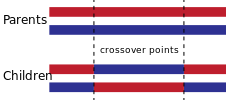
\includegraphics[width=220px]{../images/TwoPointCrossover}
\caption{Detalle operador de Cruce OX2 \label{cruce_ox_2}}
\end{figure}


\subsubsection{Operador de Mutación}

\bigskip
El \textbf{operador de mutación} intercambia entre dos elementos de la permutación. De forma aleatoria se elige si se mutará cada uno de los hijos con una probabilidad de mutación. La probabilidad de mutación son dos parámetro de nuestro algoritmo, probabilidad por individuo y probabilidad por gen, así que pueden modificar para tratar de mejorar las soluciones.

\subsubsection{Operador de Vecino}

\subsection{Técnicas de optimización local}

\bigskip
La técnica de optimización local utilizada es una técnica \textit{2-opt} proporcionada por el profesor. En la que se va comprobando como un intercambio de genes en un individuo puede mejorar su coste asociado. El pseudo-código de esta optimización es:

\begin{lstlisting}
S = candidato inicial con coste c(S) 
do {
	mejor = S
	for i=1..n
		for j=i+1..n
			T = S tras intercambiar i con j 
			if c(T) < c(S)
				S=T
} while (S != mejor)
\end{lstlisting}

\subsection{Algoritmo Genético Estándar}

En primer lugar se ha implementado un algoritmo genético básico, que utiliza los operadores de selección, cruce y mutación explicados anteriormente. Este algoritmo permite, al igual que los dos siguientes, que se indiquen un número de generaciones. El algoritmo acabará después de un número de generaciones especificado.


\subsection{Algoritmo Genético variante Baldwiniana}

La diferencia de esta variante respecto a la estándar es que se aplica una optimización local a cada generación. La optimización local se aplica una vez obtenida la nueva generación (a partir de los hijos) a todos los individuos. Una vez aplicada, se guarda el mejor individuo obtenido después de la optimización. Las soluciones optimizadas \textbf{no} se usan para generar la siguiente generación.

\subsection{Algoritmo Genético variante Lamarckiana}

La única diferencia de esta variante respecto a la \texttt{Baldwininana} es que las soluciones optimizadas, en este caso, \textbf{si} se usan para generar la siguiente generación.


\subsection{Parametros}

Los parámetros que podemos ajustar son los siguentes:

\begin{itemize}

	\item \textbf{Tamaño de población}: Una población que contiene \textbf{n} soluciones al problema. Dicha población va mejorando sus soluciones generación a generación.
	\item \textbf{Número de generaciones}: Numero de veces que va a "evolucionar' nuestra población.
	\item \textbf{Número de individuos en el torneo}: El número de elementos aleatorios que se obtendrán de la población para luego extraer el mejor de ellos. 
	\item \textbf{Probabilidad de mutación del individuo}: Aunque la mutación puede ayudar a dar más variedad a la población siempre puede provocar que no se explore a fondo un espacio donde podría haber una buena solución.
	\item \textbf{Probabilidad de mutación del gen}: Una vez se comprueba si un individuo muta se vuelve a comprobar por cada gen si este muta por otro. Este número debe ser bajo ya que si no se generarían individuos muy diferentes.
\end{itemize}


